\documentclass[letterpaper, 12pt]{article}
\usepackage[margin=1in]{geometry}
\usepackage{amssymb}
\usepackage{graphicx}
\usepackage[utf8]{inputenc}
\usepackage{indentfirst}
\usepackage{physics}
\usepackage{amsmath}

%\usepackage[round]{natbib}
\usepackage{apacite}
\usepackage{url} % not crucial - just used below for the URL 


\title{\bf Title}
\author{Cristy\\ F bio, Universidad Autónoma de Coahuila,\\ Torreón, México.
	\and
	Nagamani \\
	F bio WWW, Universidad Autónoma de Coahuila
	\and
	Raji \\
	Department of ZZZ, University of WWW
	\and
	S. K. Gadi\thanks{Author to whom all correspondence should be addressed.} \\
	%Facultad de Ingeniería Mecánica y Eléctrica,\\ 
	FIME, Universidad Autónoma de Coahuila,\\ Torreón, México.
}


\providecommand{\keywords}[1]{\textbf{\textit{Index terms---}} #1}

\begin{document}
	\maketitle
	\begin{abstract}
		One of the challenges in teaching the subject Design of Experiments is to come up with a proper numerical example. In this article, authors present a methodology to generate a numerical example for multifactorial experiments. Also, it presents a simple algorithm, which can be implemented in any programming language to generate unique models.
	\end{abstract}
	\keywords{Experimental design; educational tool; generating examples}
	\section{Introduction}
	The subject experimental design is part of various undergraduate and graduate curriculum, ranging from the engineering to the biological sciences. Learning statistics or mathematics in general is effective by solving a number of numerical examples. It is teacher's task to generate them \cite{Deborah2008}.
	\par
	Teachers spend a lot of time in generating an appropriate examples, which meet all the characteristics they want to highlight. In this article we present a methodology to generate such example for the subject experimental design. The algorithm is described in the section ((???)). Readers interested only in the implementation of algorithm may skip the mathematical construction presented in the section ((???)).
	\par
	One of the objectives in the experimental design is to find the factors which optimize the responses of a physical process. Solving problems in this subject involves performing various experiments with a different combinations of factors. Conducting experiments on a real system for the classroom purpose is not always feasible due to any the following limitations.
	\begin{enumerate}
		\item The cost of conducting experiments on a real system is not always negligible.
		\item A considerable amount of time may take for each experiment.
		\item The combination of factor associated for optimum response is constant for a physical system. Therefore, teachers may not provide a fresh problem.
	\end{enumerate}
	\par
	A computer program generating responses is a good alternative to mimic the physical systems. Hence, a numerical example for an experimental design is mathematical model representing a physical process. This model is a set of static functions (i.e. it does not have derivative or integral terms) which maps the factors to the responses. A multi-response system can be represented as
	\begin{eqnarray}
	y_i &=& f_i(x_1, x_2, x_3, \dots, x_n) + \xi_i \label{Eqn:Function}
	\end{eqnarray}
	\noindent where $y_i$, $i\in \{1,2,3, \dots, m\}$ are the responses, $x_j$, $j\in \{1,2,3, \dots, n\}$ are the factors, $f_i$, $i\in \{1,2,3, \dots, m\}$ are the nonlinear functions mapping the $n$ factors to the $m$ responses and $\xi_i$, $i\in \{1,2,3, \dots, m\}$ are the noise.
	\par
	All the factors, $x_j$, are constrained by upper and lower limits. The numerical examples should produce an unique optimal responses, $y_i$, for a set of factors within its limits. Also, it should be guaranteed that there exists no other peaks in the surface. A convex function meets our requirements. Construction of a one such mathematical function is presented in the next section.
	\section{Construction of an convex function to suit our requirements}
	\subsection{Quadratic convex function}
	\begin{figure}
		\centering
		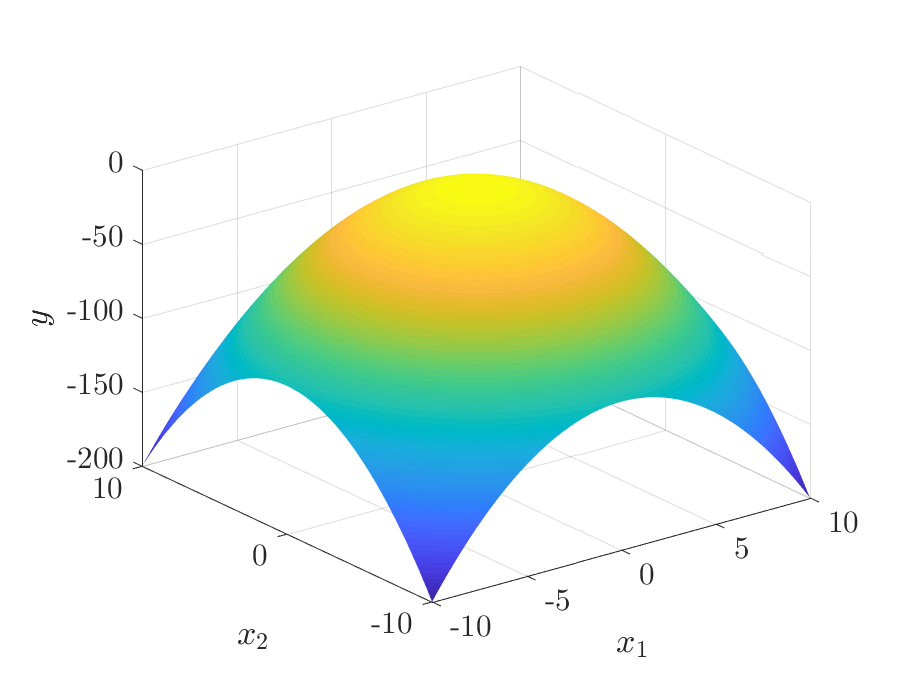
\includegraphics[width=0.75\textwidth]{Matlab/poly-2-var}
		\label{Fig:TwoVariablePolynomial}
		\caption{A second order polynomial convex function}
	\end{figure}
	A second order polynomial function, such as
	\begin{eqnarray}
	y_i &=& -\sum_{i=1}^{i=n}{x_i^2} \label{Eqn:PolyFunction}
	\end{eqnarray}
	is a convex function, which serve the purpose of providing a unique optimal point. Figure~\ref{Fig:TwoVariablePolynomial} depicts (\ref{Eqn:PolyFunction}) for the two variables case. However, it doesn't represent a real physical system due to the following limitations.
	\begin{enumerate}
		\item Response surface methodology uses a second order fit algorithm. Hence, the process of reaching optimal solution becomes trivial.
		\item A quadratic function is having a property that its slope increases as it moves far from the optimal point. This property trivializes the process of selecting a new base value.
	\end{enumerate}
	\subsection{Sigmoid convex function}
	\begin{figure}
		\centering
		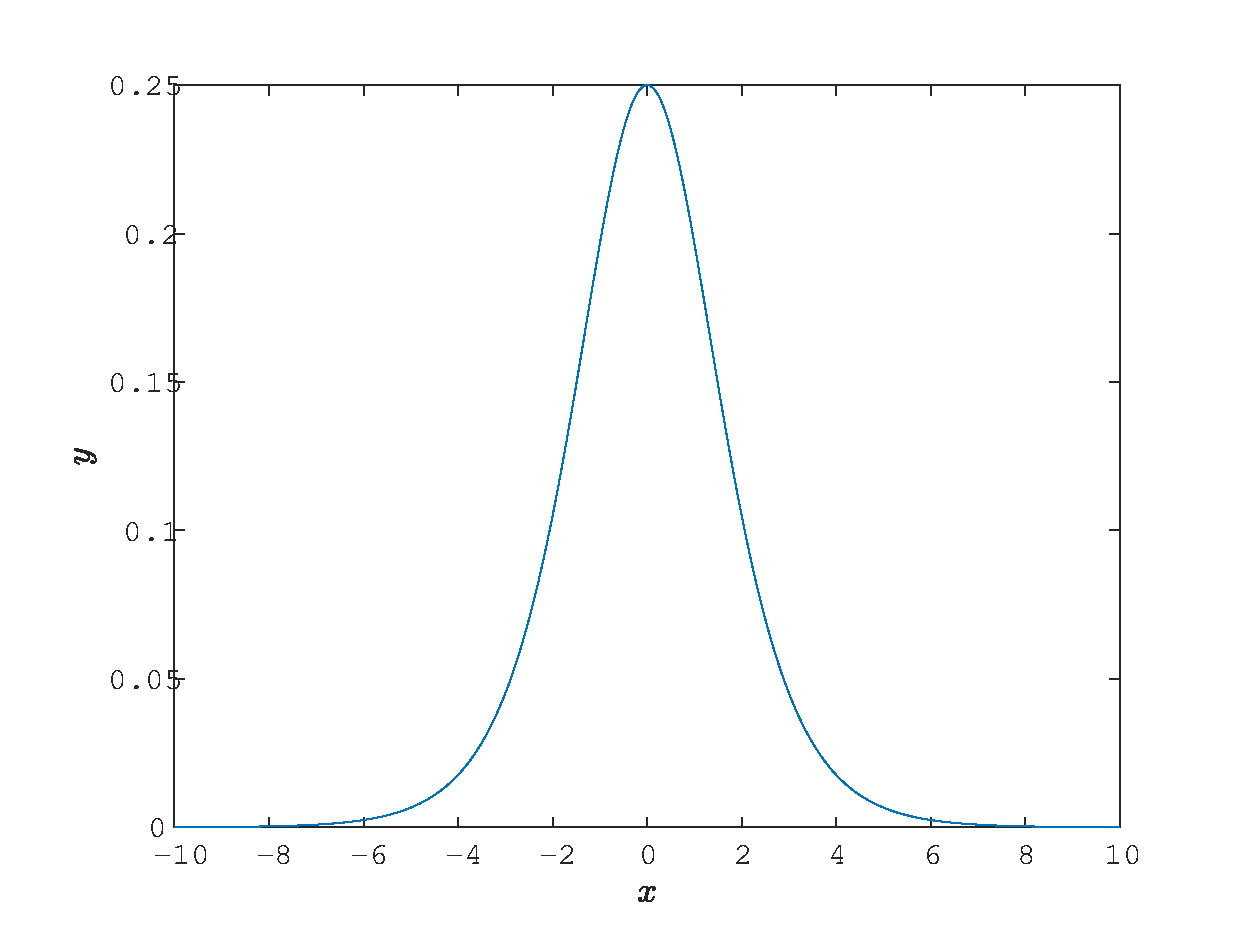
\includegraphics[width=0.75\textwidth]{Matlab/1FactorsSigmoid}
		\label{Fig:OneVarSigmoid}
		\caption{One variable convex function}
	\end{figure}
	\begin{figure}
		\centering
		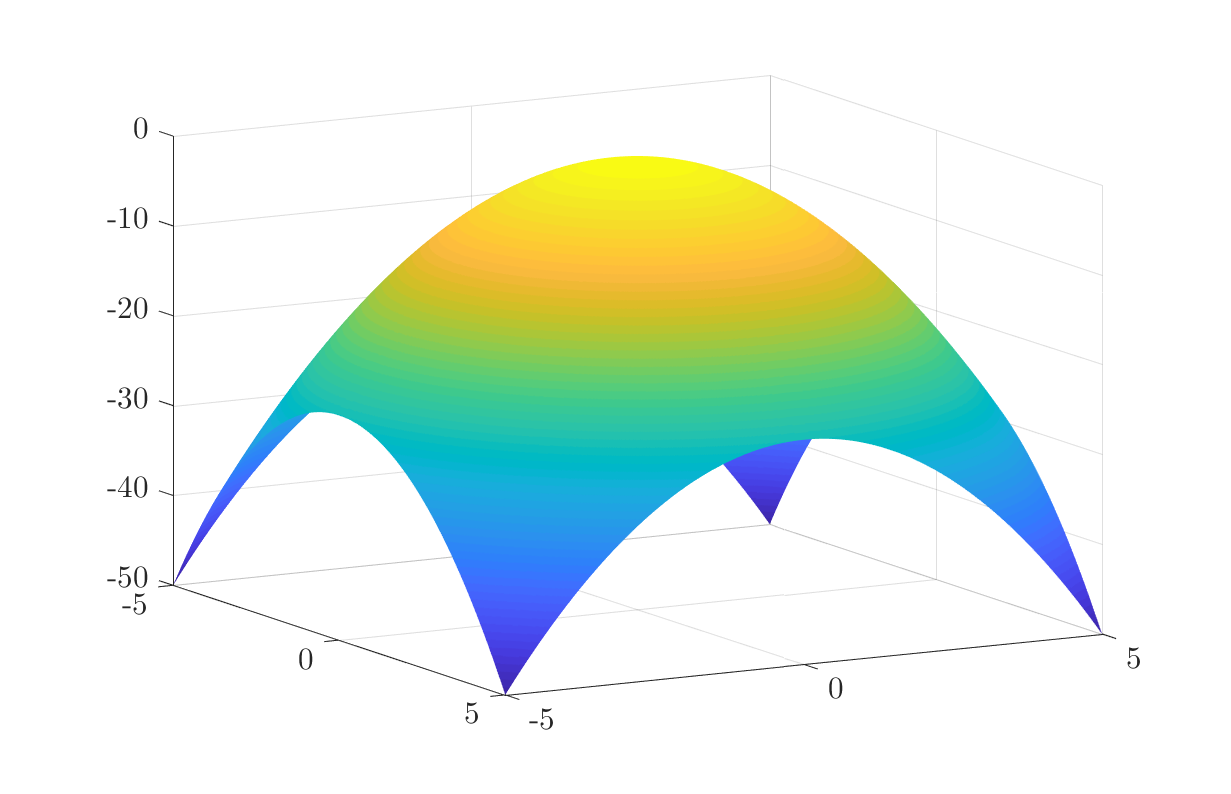
\includegraphics[width=0.75\textwidth]{Matlab/2FactorsSigmoid}
		\label{Fig:MultiVarSigmoid}
		\caption{Two variable convex function}
	\end{figure}
	Keeping above limitation in mind, a sigmoid based convex function is proposed. One variable sigmoid function is
	\begin{eqnarray}
	S(x) = \frac{1}{1-e^{-x}} \label{Eqn:Sigmoid}
	\end{eqnarray}
	and its derivative is
	\begin{eqnarray}
	S_d(x) = S'(x) = \frac{e^x}{(e^{x}+1)^2} = S(x)(1-S(x)). \label{Eqn:DiffSigmoid}
	\end{eqnarray}
	\par
	The function $S_d$ addresses limitations of mentioned in the previous sub-section. The function $S_d$ is plotted in Figure~\ref{Fig:OneVarSigmoid}. The function $S_d$ can be extended to a $n$ variables case as
	\begin{eqnarray}
	S_d(x_1, x_2, x_3, ..., x_n) = \sum_{i=1}^{i=n}{\frac{e^x_i}{(e^{x_i}+1)^2}}. \label{Eqn:DiffSigmoidMulti}
	\end{eqnarray}
	\par
	Figure~\ref{Fig:MultiVarSigmoid} shows sigmoid based function for two variables. Hessian matrix for $S_d(x_1, x_2, x_3, ..., x_n)$ is 
	\begin{eqnarray}
	H_{i,j} = 
	\begin{cases}
	\pdv[2]{S_d}{x_i},& \text{if } i = j\\
	0,              & \text{otherwise}
	\end{cases}
	= asflkasjflaksjflksfj \label{Eqn:HessianMatrix}
	\end{eqnarray}
	\par
	The Hessian matrix, $H_{i,j}$ is having a positive definate because it is a diagonal matrix and the diagnal values are positive. Hence, $S_d$ is a convex function, i.e. has a unique maximum value with no other peaks. In the next section a method is presented to adapt $S_d$ to generate random experiments within given limits.
	\section{Adapting convex function}
	It can be observed that the convex function, $S_d$, proposed in the previous section has a maximum value at $x_i=0, \forall i\in\{1, 2, 3, \dots, n\}$ and a value close to zero for $x_i>5, \forall i\in\{1, 2, 3, \dots, n\}$
	
	
	
	
	
	\bibliographystyle{apacite}%unsrtnat}
	\bibliography{refs}
\end{document}
